%!TEX root = ../../master.tex

\section{Physical Design}
The physical design of KubeCloud is very important in order to satisfy the requirements. The process of building and designing the cluster started out with sketching the possible physical designs. After the initial process of sketching, 3D models of the cluster with the components were made to visualize the cluster and compare it to images of real datacenters. Lastly, an exact 3D model of the individual parts needed to be manufactured was created and sent to the fabricator. The process of the physical design can be seen in Figure~\ref{fig:design_process}.

% SKETCH, 3D, CLUSTER
\begin{figure}[H]%
    \centering
    \subfloat[Sketch]{{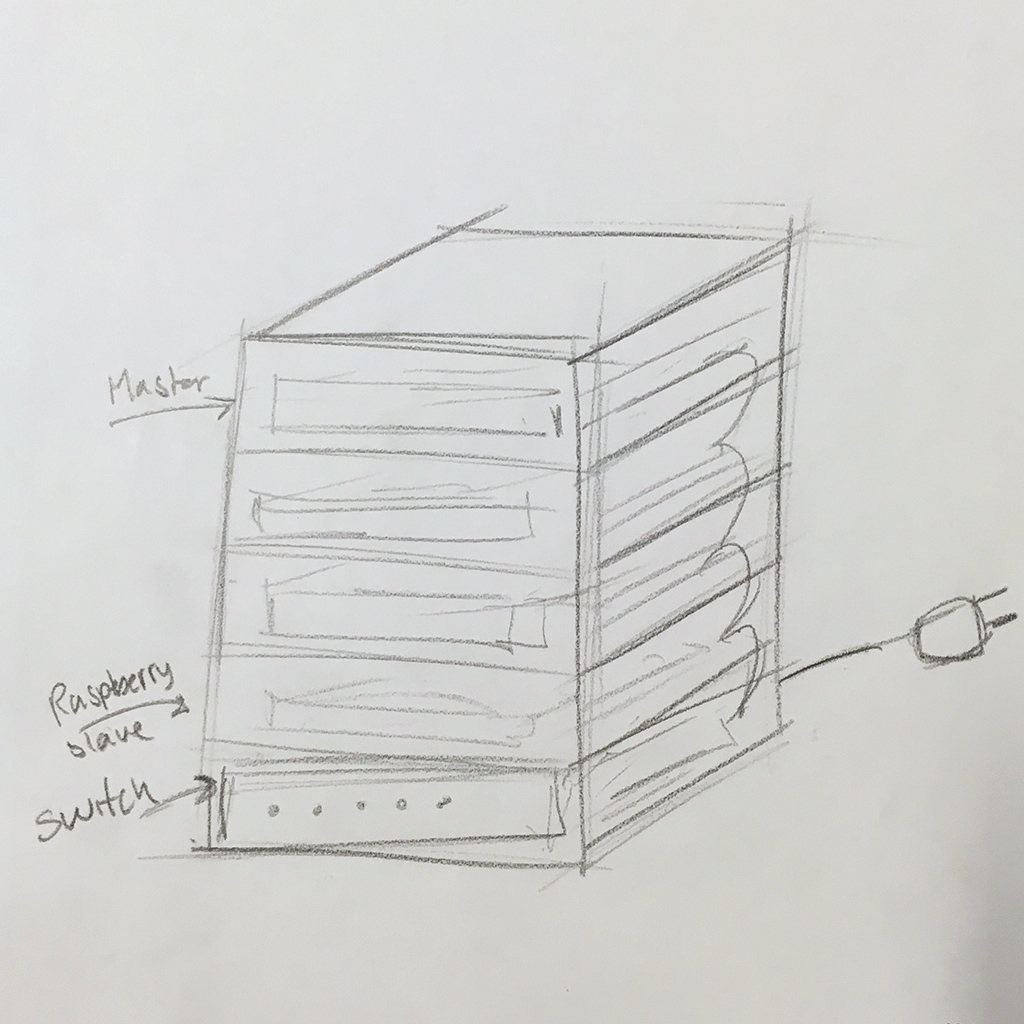
\includegraphics[width=4cm]{figures/cluster/sketch} }}%
    \qquad
    \subfloat[3D model]{{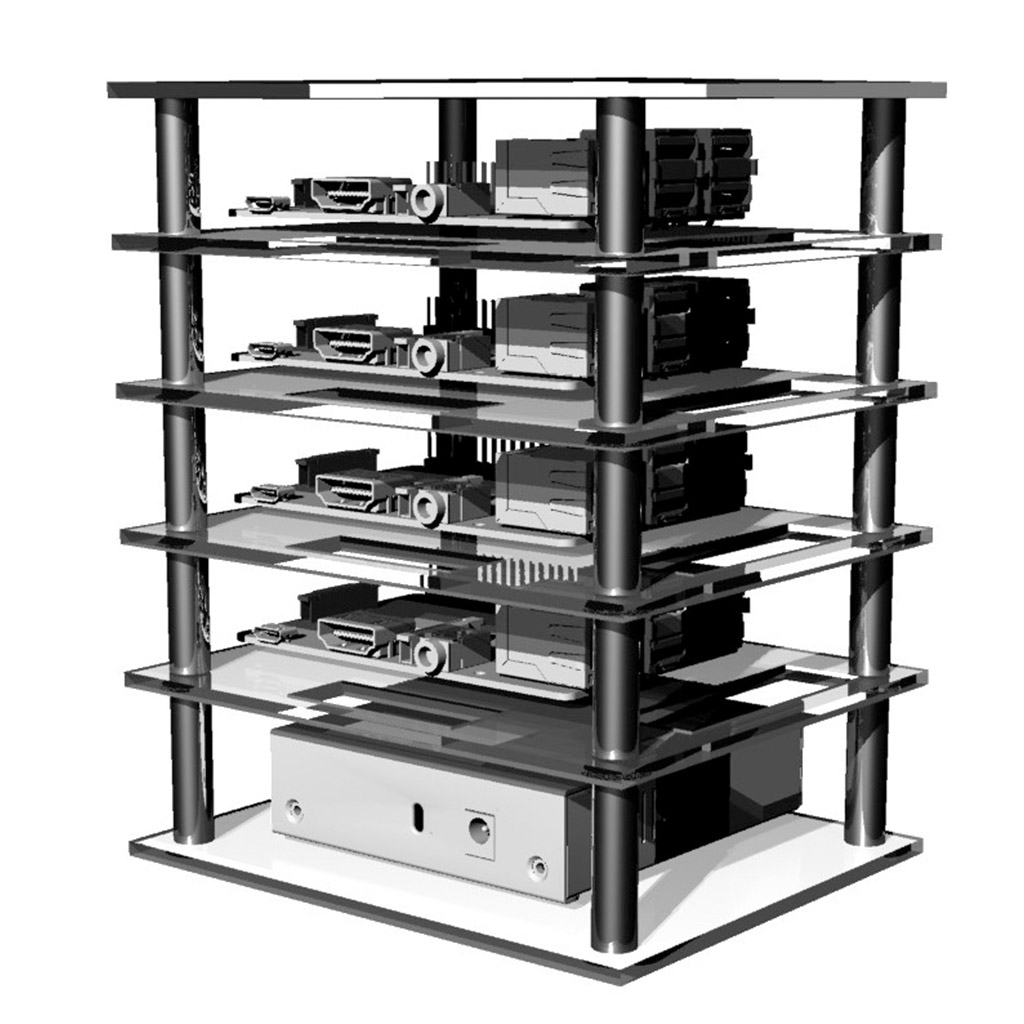
\includegraphics[width=4cm]{figures/cluster/cluster3d_back} }}%
    \qquad
    \subfloat[KubeCloud]{{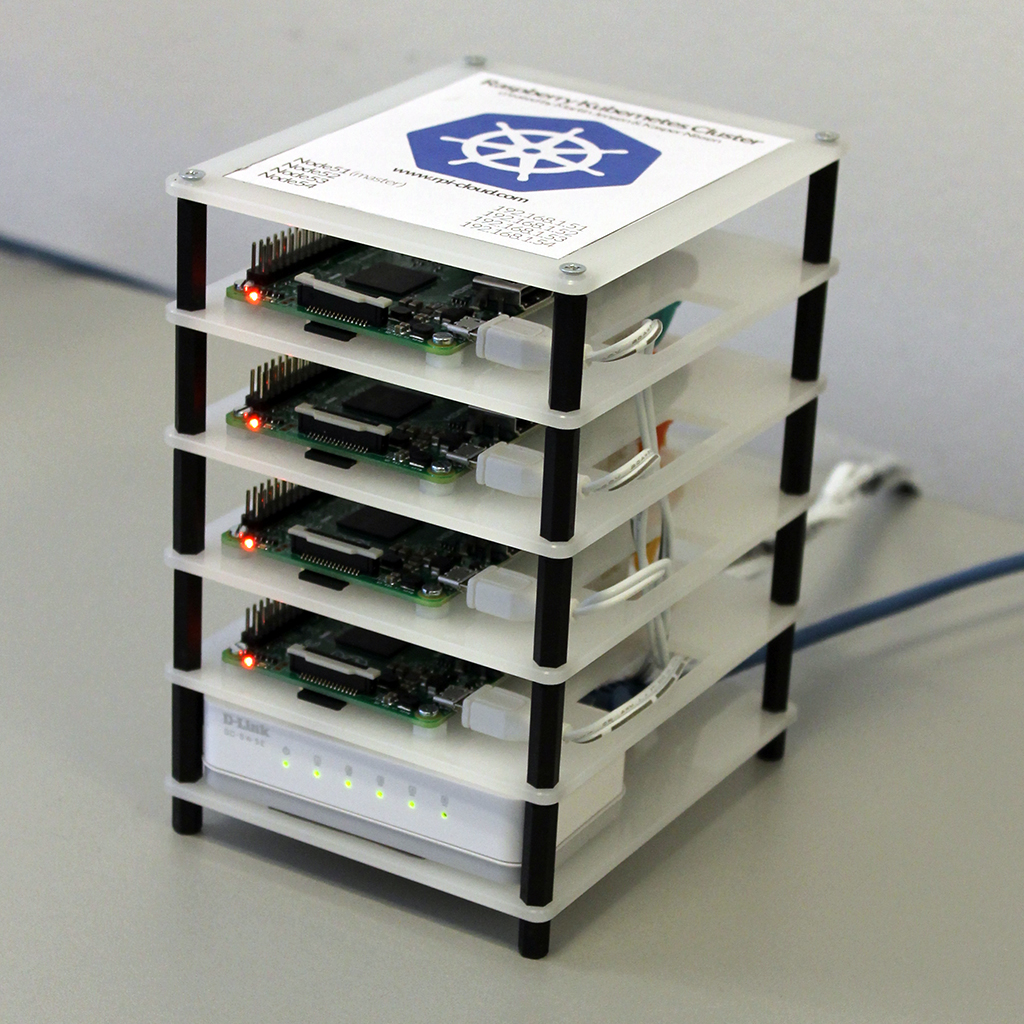
\includegraphics[width=4cm]{figures/cluster/kubecloud_alone} }}%
   
    \caption{Sketch, 3D, and Cluster}%
    \label{fig:design_process}%
\end{figure}

\noindent
The requirement \textit{"KubeCloud shall visually have characteristics of a server rack"} should afford visual associations of working on a scale-model of a data center. KubeCloud consists of stackable layers of Raspberry Pis similar to servers stacked in a server rack in a real data center. Figure~\ref{fig:server_rack} shows the similarity between a server rack and KubeCloud. 

% RACK VS CLUSTER
\begin{figure}[H]%
    \centering
    \subfloat[Rack]{{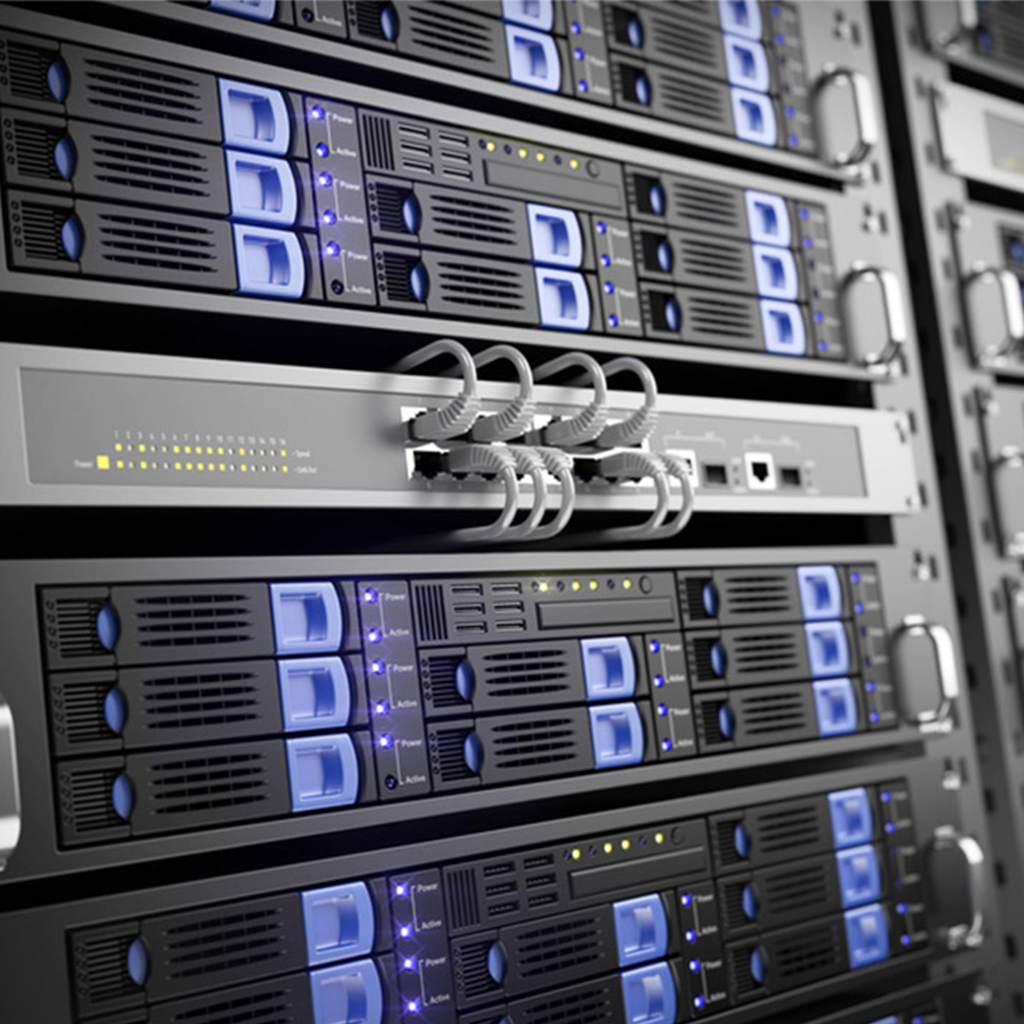
\includegraphics[width=4cm]{figures/cluster/rack} }}%
    \qquad
    \subfloat[KubeCloud]{{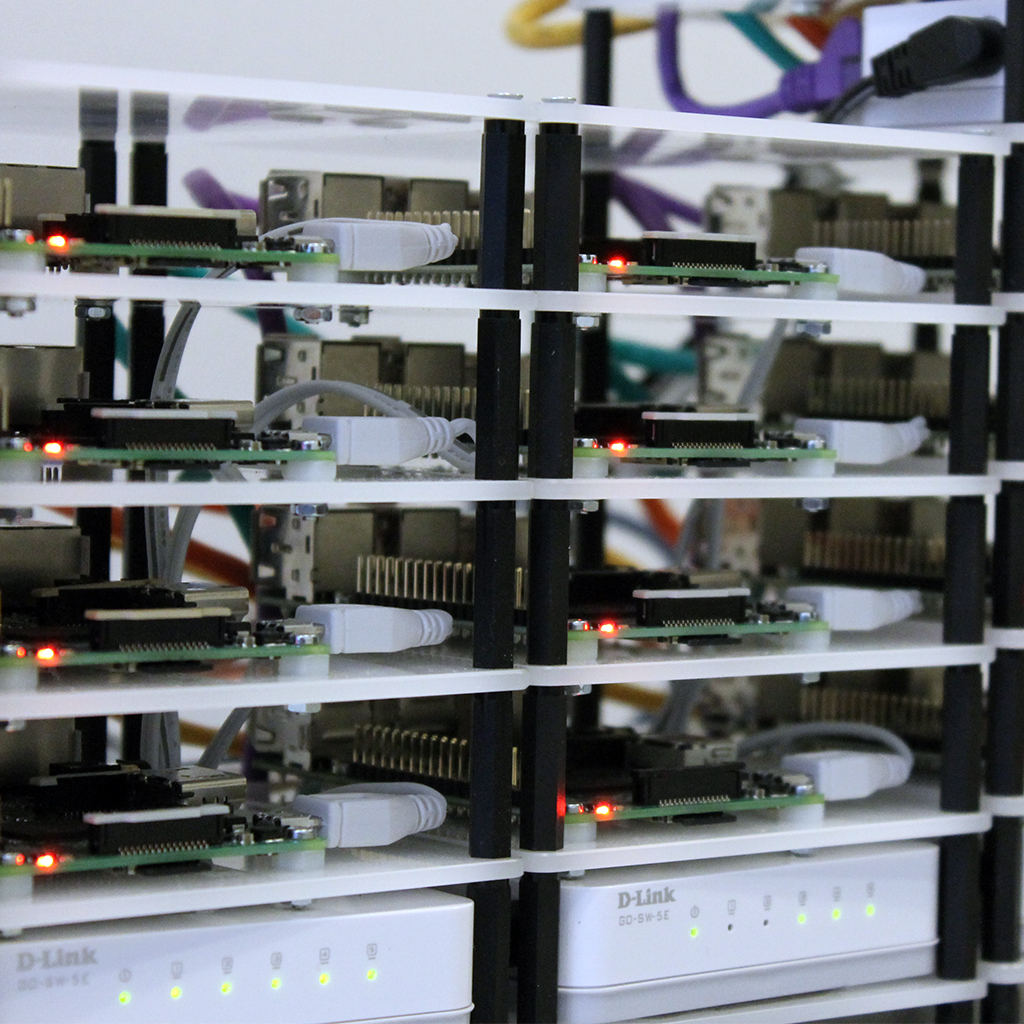
\includegraphics[width=4cm]{figures/cluster/kubecloud_rack} }}%
    \qquad
    \subfloat[KubeCloud]{{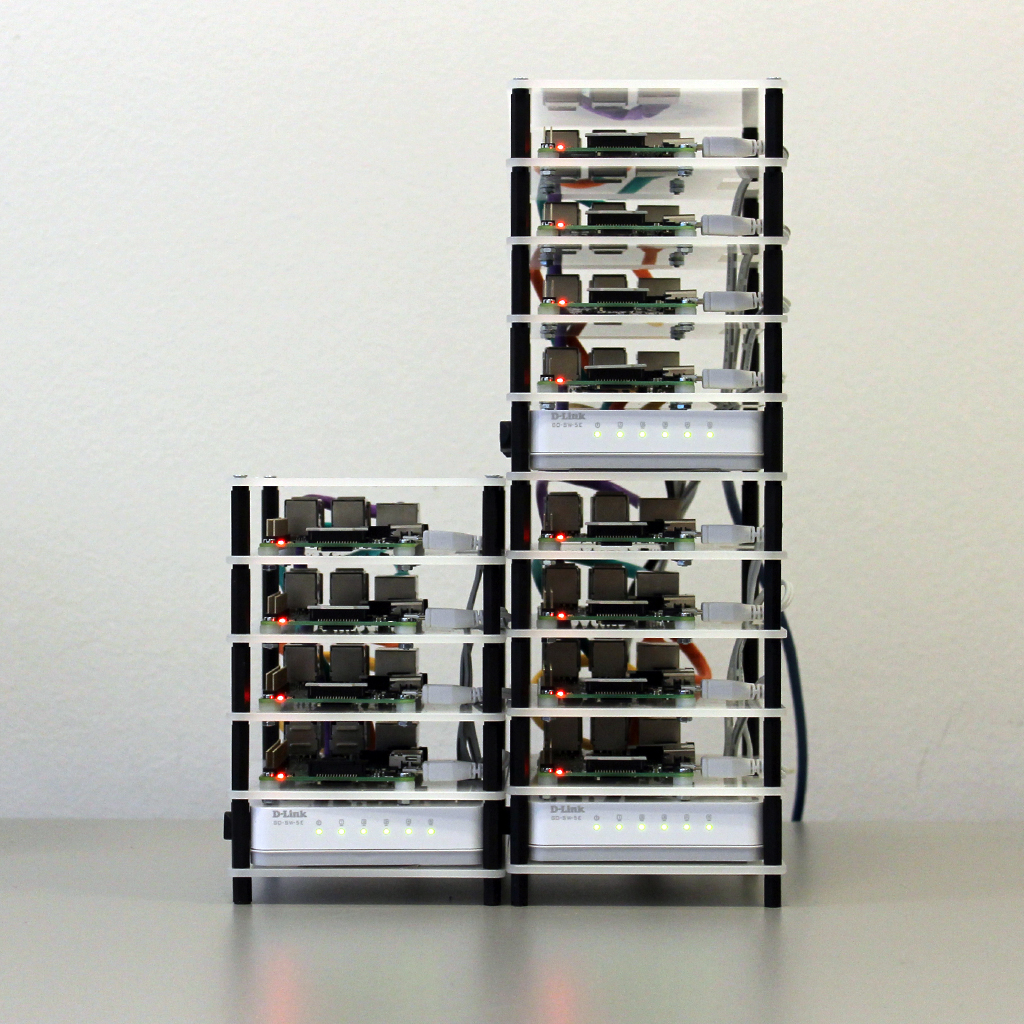
\includegraphics[width=4cm]{figures/cluster/kubecloud_high} }}%
    \caption{Rack Versus Cluster}%
    \label{fig:server_rack}%
\end{figure}

\noindent
Figure~\ref{fig:server_rack} (a) shows a real server rack in a data center. Figure~\ref{fig:server_rack} (b) shows multiple KubeClouds comprising a larger scale data center compared to a single KubeCloud. Figure~\ref{fig:server_rack} (c) shows the dynamism of KubeCloud and the ability to configure the cluster size from a physical perspective. Multiple KubeClouds can easily be mounted together to form a larger small-scale cloud computing environment. This satisfies the requirement of \textit{"KubeCloud shall allow for configuration of the cluster size"}. \\

\noindent
To satisfy the requirement of \textit{"KubeCloud shall have a small physical form factor and be able to be carried around in a bag"}, the power and network connectors are enclosed in the body of the physical design in order to avoid damage during transportation. This further satisfies the requirement \textit{"KubeCloud shall be transportable"}.
The physical size of KubeCloud is made as small as possible within the constraints of the size of the used components (Raspberry Pi and dlinkgo) and the concealment of cables. Figure~\ref{fig:technical_drawings} shows the technical drawings of the two different layers the cluster is comprised of. (a) is the layer the Raspberry Pi is mounted on, (b) is the top and the bottom layer. The 3D model of the two layers can be downloaded from our blog\footnote{\url{http://rpi-cloud.com/guide-how-to-build-a-raspberry-pi-cluster/}}.

% TECHNICAL DRAWINGS
\begin{figure}[H]%
    \centering
    \subfloat[Raspberry Pi layer]{{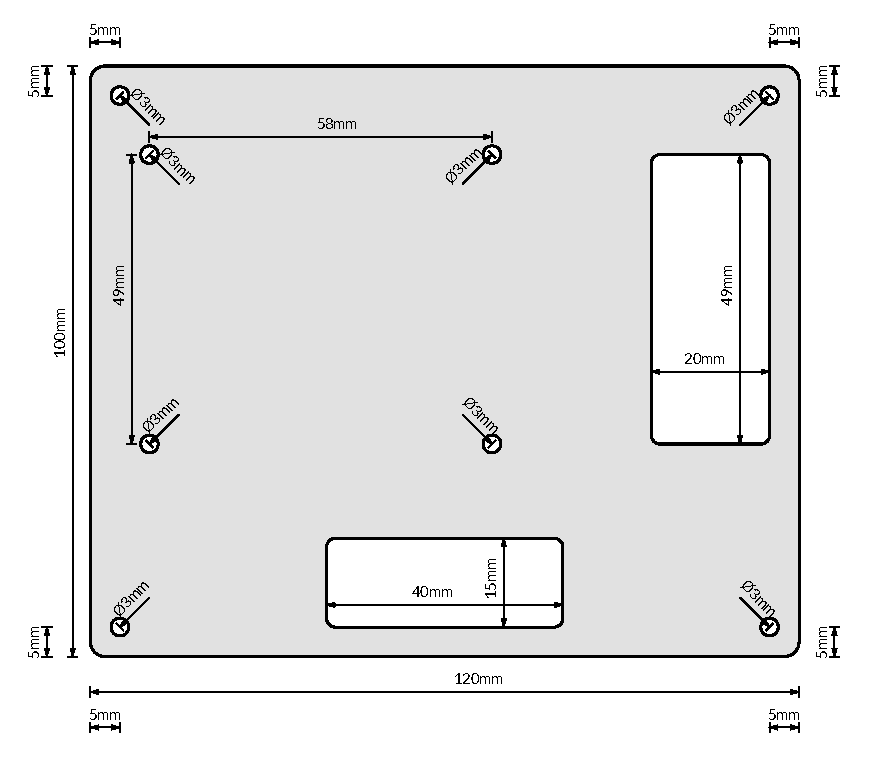
\includegraphics[width=6.5cm]{figures/cluster/raspberry_layer} }}%
    \qquad
    \subfloat[Top bottom layer]{{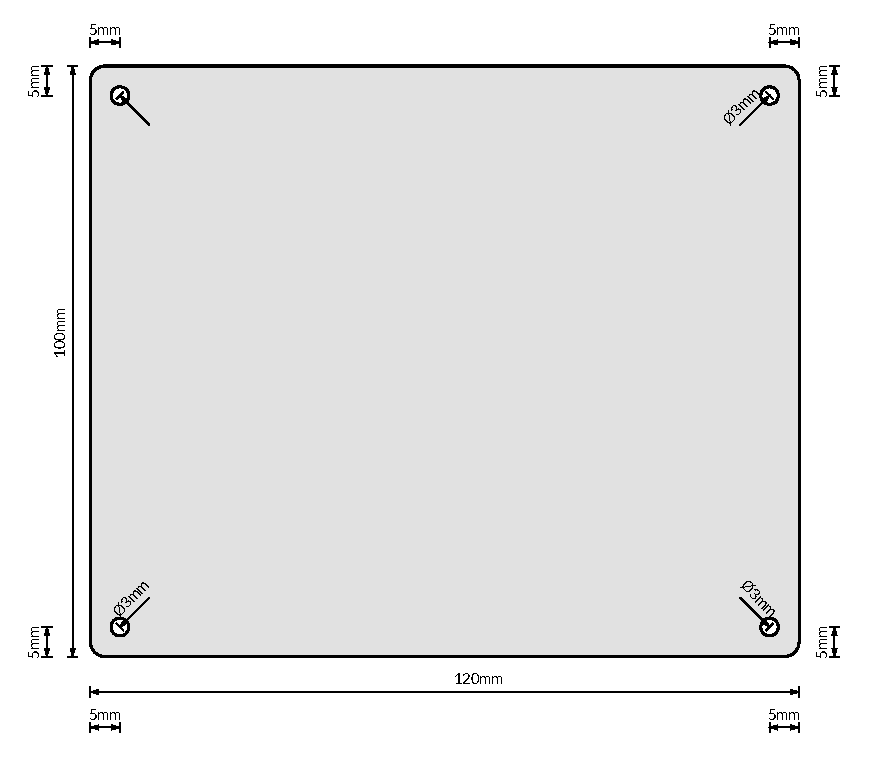
\includegraphics[width=6.5cm]{figures/cluster/top_bottom_layer} }}%
    \caption{Technical Drawings 1:2.5}%
    \label{fig:technical_drawings}%
\end{figure}

\noindent
One of the important purposes of KubeCloud is to demonstrate the effect of failures e.g. network failure. The hole, seen on the right side of Figure~\ref{fig:technical_drawings} (a), makes the ethernet port of the Raspberry Pi accessible and allows for pulling the plug through this hole. This satisfies the requirement of \textit{"KubeCloud shall allow students to pull out cables to inject failures"}.
